% Documentclass options:
%    10pt, 11pt, 12pt  -- set type size
%    draft             -- single space, mark overfull hboxes on paper
%    final             -- double space, don't mark overfull hboxes on paper
%    oneside           -- format for one-sided printing
%    twoside           -- format for two-sided printing
% Defaults are 11pt,final,oneside.  Keep these, please.
\documentclass[11pt]{ucscthesisbs}
\bibliographystyle{apalike2}
\usepackage{natbib}
\usepackage{graphicx,epsf}% Include figure files


% The following declaration is for citations and bibliographies consistent with
% Astrophysical Journal specifications.  It may be left out or replaced with
% another bibliography/citation style.  See also the "\bibliographystyle"
% command later in this file.
%\usepackage{apj}

\usepackage{xcolor}
\usepackage{pagecolor}
\usepackage{lipsum}  
\usepackage{subfig}
\usepackage{amsmath}
\usepackage[font=small,labelfont=bf]{caption}

\pagecolor{darkgray}
\color{white}

% \pagecolor{white}
% \color{black}


\begin{document}

% Declarations for Front Matter

\title{Thermal Evolution of Uranus and Neptune with Condensation-inhibited Convection}
\author{Robert Schroder}
\degreeyear{2020}
\degreemonth{November}
\degree{BACHELOR OF SCIENCE}
\field{ASTROPHYSICS}%
% Declare up to five committee members.  The text will be reproduced directly
% on the signature page.  Though the chair is a committee member, leave
% him/her out of the \committeemember declarations.  Make sure \numberofmembers
% agrees with the number of committee members declared INCLUDING the chair.
% If it is wrong, you will get extra or missing lines on the signature page.
%
\chair{Bruce Schumm}
\thesisadvisor{Christopher Mankovich}
\technicaladvisor{Jonathan Fortney}
\numberofmembers{2}




\campus{Santa Cruz}

\maketitle
\copyrightpage

\begin{frontmatter}

\begin{abstract}
This will be the last section written, once we have finished our results and conclusion.
\end{abstract}

\tableofcontents
%
% The most recent (10/95) guidelines make absolutely no mention of the list
% of figures and list of tables.  Are they necessary?  If not, comment the
% next two lines out.
%
\listoffigures
\listoftables

\begin{dedication}
\null\vfil
{\large
\begin{center}
To Who,\\\vspace{12pt}
M  ention to who, if anyone, here
\end{center}}
\vfil\null
\end{dedication}

\begin{acknowledgements}
I'd like to thank....
\end{acknowledgements}


\end{frontmatter}

%\part{First Part}

\chapter{Introduction}
Observations of Uranus show a planet that appears to be in thermal equilibrium with the Sun. Observation has also shown that Uranus is cooler than its more distant neighbor, Neptune. Thermal evolution models for Uranus have not matched observation, instead predicting a warmer effective temperature during the current epoch\citep{fortney_2011}, \citep{podolak_1991}, \citep{hubbard_1995}, \citep{scheibe_2019} [There are other papers by Nettelmann 2013, Linder 2019 that I haven't looked at yet]. 

There have been various attempts to explain the underluminous Uranus. The formation of stable layers, trapping internal energy in the the interior of Uranus and Neptune was proposed by \citep{podolak_1991}. There has also been much work done investigating the formation of stable condensation zones that inhibit convection \citep{friedson_2017}, \citep{leconte_2017}, and \citep{guillot_1995}. 


\chapter{Model}

\section{Theoretical Foundations for Fully Convective, Dry Interior}
Underlying the model are mathematics and physics dating back to the first attempts to model the thermal evolution of giant planets \citep{hubbard_1977} and later attempts to model Uranus and Neptune \citep{hubbard_1977_2} and \citep{podolak_1991}. We begin with conservation of mass:

\begin{equation}
  \frac{dm}{dr} =4 \pi r^{2}\rho  
\end{equation}
where $dm$ is the mass contained within a sphere of radius $r$. $\rho(r)$ is the density at radius $r$. We also assume hydrostatic equilibrium, given by:

\begin{equation}
  \frac{dP}{dr} = -\frac{Gm\rho}{r^{2}}  
\end{equation}
where $P$ is the pressure and $G$ is the gravitational constant. For onservation of energy and the thermal evolution of the planet, we relate the intrinsic luminosity profile $L(m)$ to the rate of change of specific entropy $s$ in the planet as follows:

\begin{equation}
  \frac{dL}{dm}=-T\frac{\delta s}{\delta t}.
\end{equation}
Integrating over the mass of the planet and solving for the timestep, $\delta t$, yields

\begin{equation}
  \delta t=-\frac{1}{L_{\rm int}}\int_0^M T\,\delta s\,dm
\end{equation}
where $L_{\rm int}$ is the intrinsic luminosity, given by:

\begin{equation}
  L_{\rm int} = 4\pi r^{2}\sigma_{\rm SB}T_{\rm int}^{4}
\end{equation}

Furthermore, for our base comparison model, we assume a standard three-layer structure for Uranus and Neptune as seen in Figure 2.1. At the center of the planet is a core made of ??. The inner envelope is $H_{2}O$ dominated, with uniform concentrations of $H$, $He$, and $H_{\rm{2}}O$, using the MAZEVET EOS \citep{mazevet_2019}. The outer envelope, below 10 bars, contains trace amounts of $H_{\rm{2}}O$, but is mostly $H$ and $He$, dominated, and utilizes the MH13SCVH EOS \citep{miguel_2018}. Both  inner and outer envelopes are fully convective, with the pressure-temperature profile following a dry adiabat, given by $\nabla_{\rm ad}$:

\begin{equation}
T(P>P_{\rm base}) = T_{\rm base} + \int_{P_{\rm base}}^P\left(\frac{dT}{dP}\right)_{\rm ad}\,d P
\end{equation}

\begin{figure}[ht!]
 \centerline{
  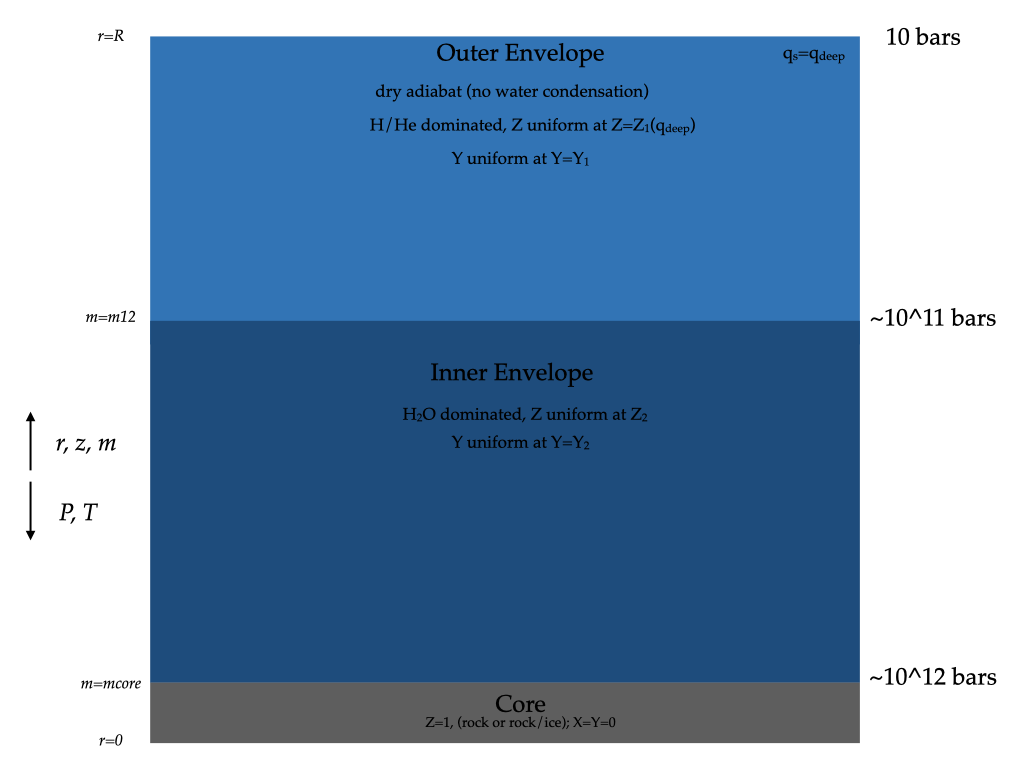
\includegraphics[width=6.0in]{figures/structure_schematic_images/structure_schematic_images.001.png}
 }
\caption[A Standard Interior Structure Model]
{The structure for a fully convective, dry adiabatic interior.}
\label{fig:standard_dry_interior}
\end{figure}


Finally, beyond the outer envelope is the atmosphere. When modeling the thermal evolution of gas and ice giants, it has long been recognized that model atmospheres constitute an outer boundary condition for interior structure models, providing key inputs that impact cooling times for interior structure models. Our work considers both \citep{graboske_1975} and \citep{fortney_2011} model atmospheres. Unless otherwise stated, our results will utilize the Fortney 2011 model atmospheres. 


\section{Addition of a Moist Adiabat to the Outer Envelope with Condensation-inhibited Convection}
Our interior structure model departs from the standard model described above by adding a moist adiabatic layer to the outer envelope. In our case, this allows for the condensation of water. We do not account for other condensates such as $CH_{4}$ and $NH_{3}$.

As seen in Figure (Y).   Within the outer envelope, we implement moist adiabatic layer, such that when conditions are suitable for condensation, we allow for the formation of a stable water condensation zone. ADD PHYSICS FOR CONDENSATION (Include equations for $q_{s}$, latent heat, xi, saturation vapor pressure, ... other equations that define the moist adiabat.)

\begin{figure}[ht!]
 \centerline{
  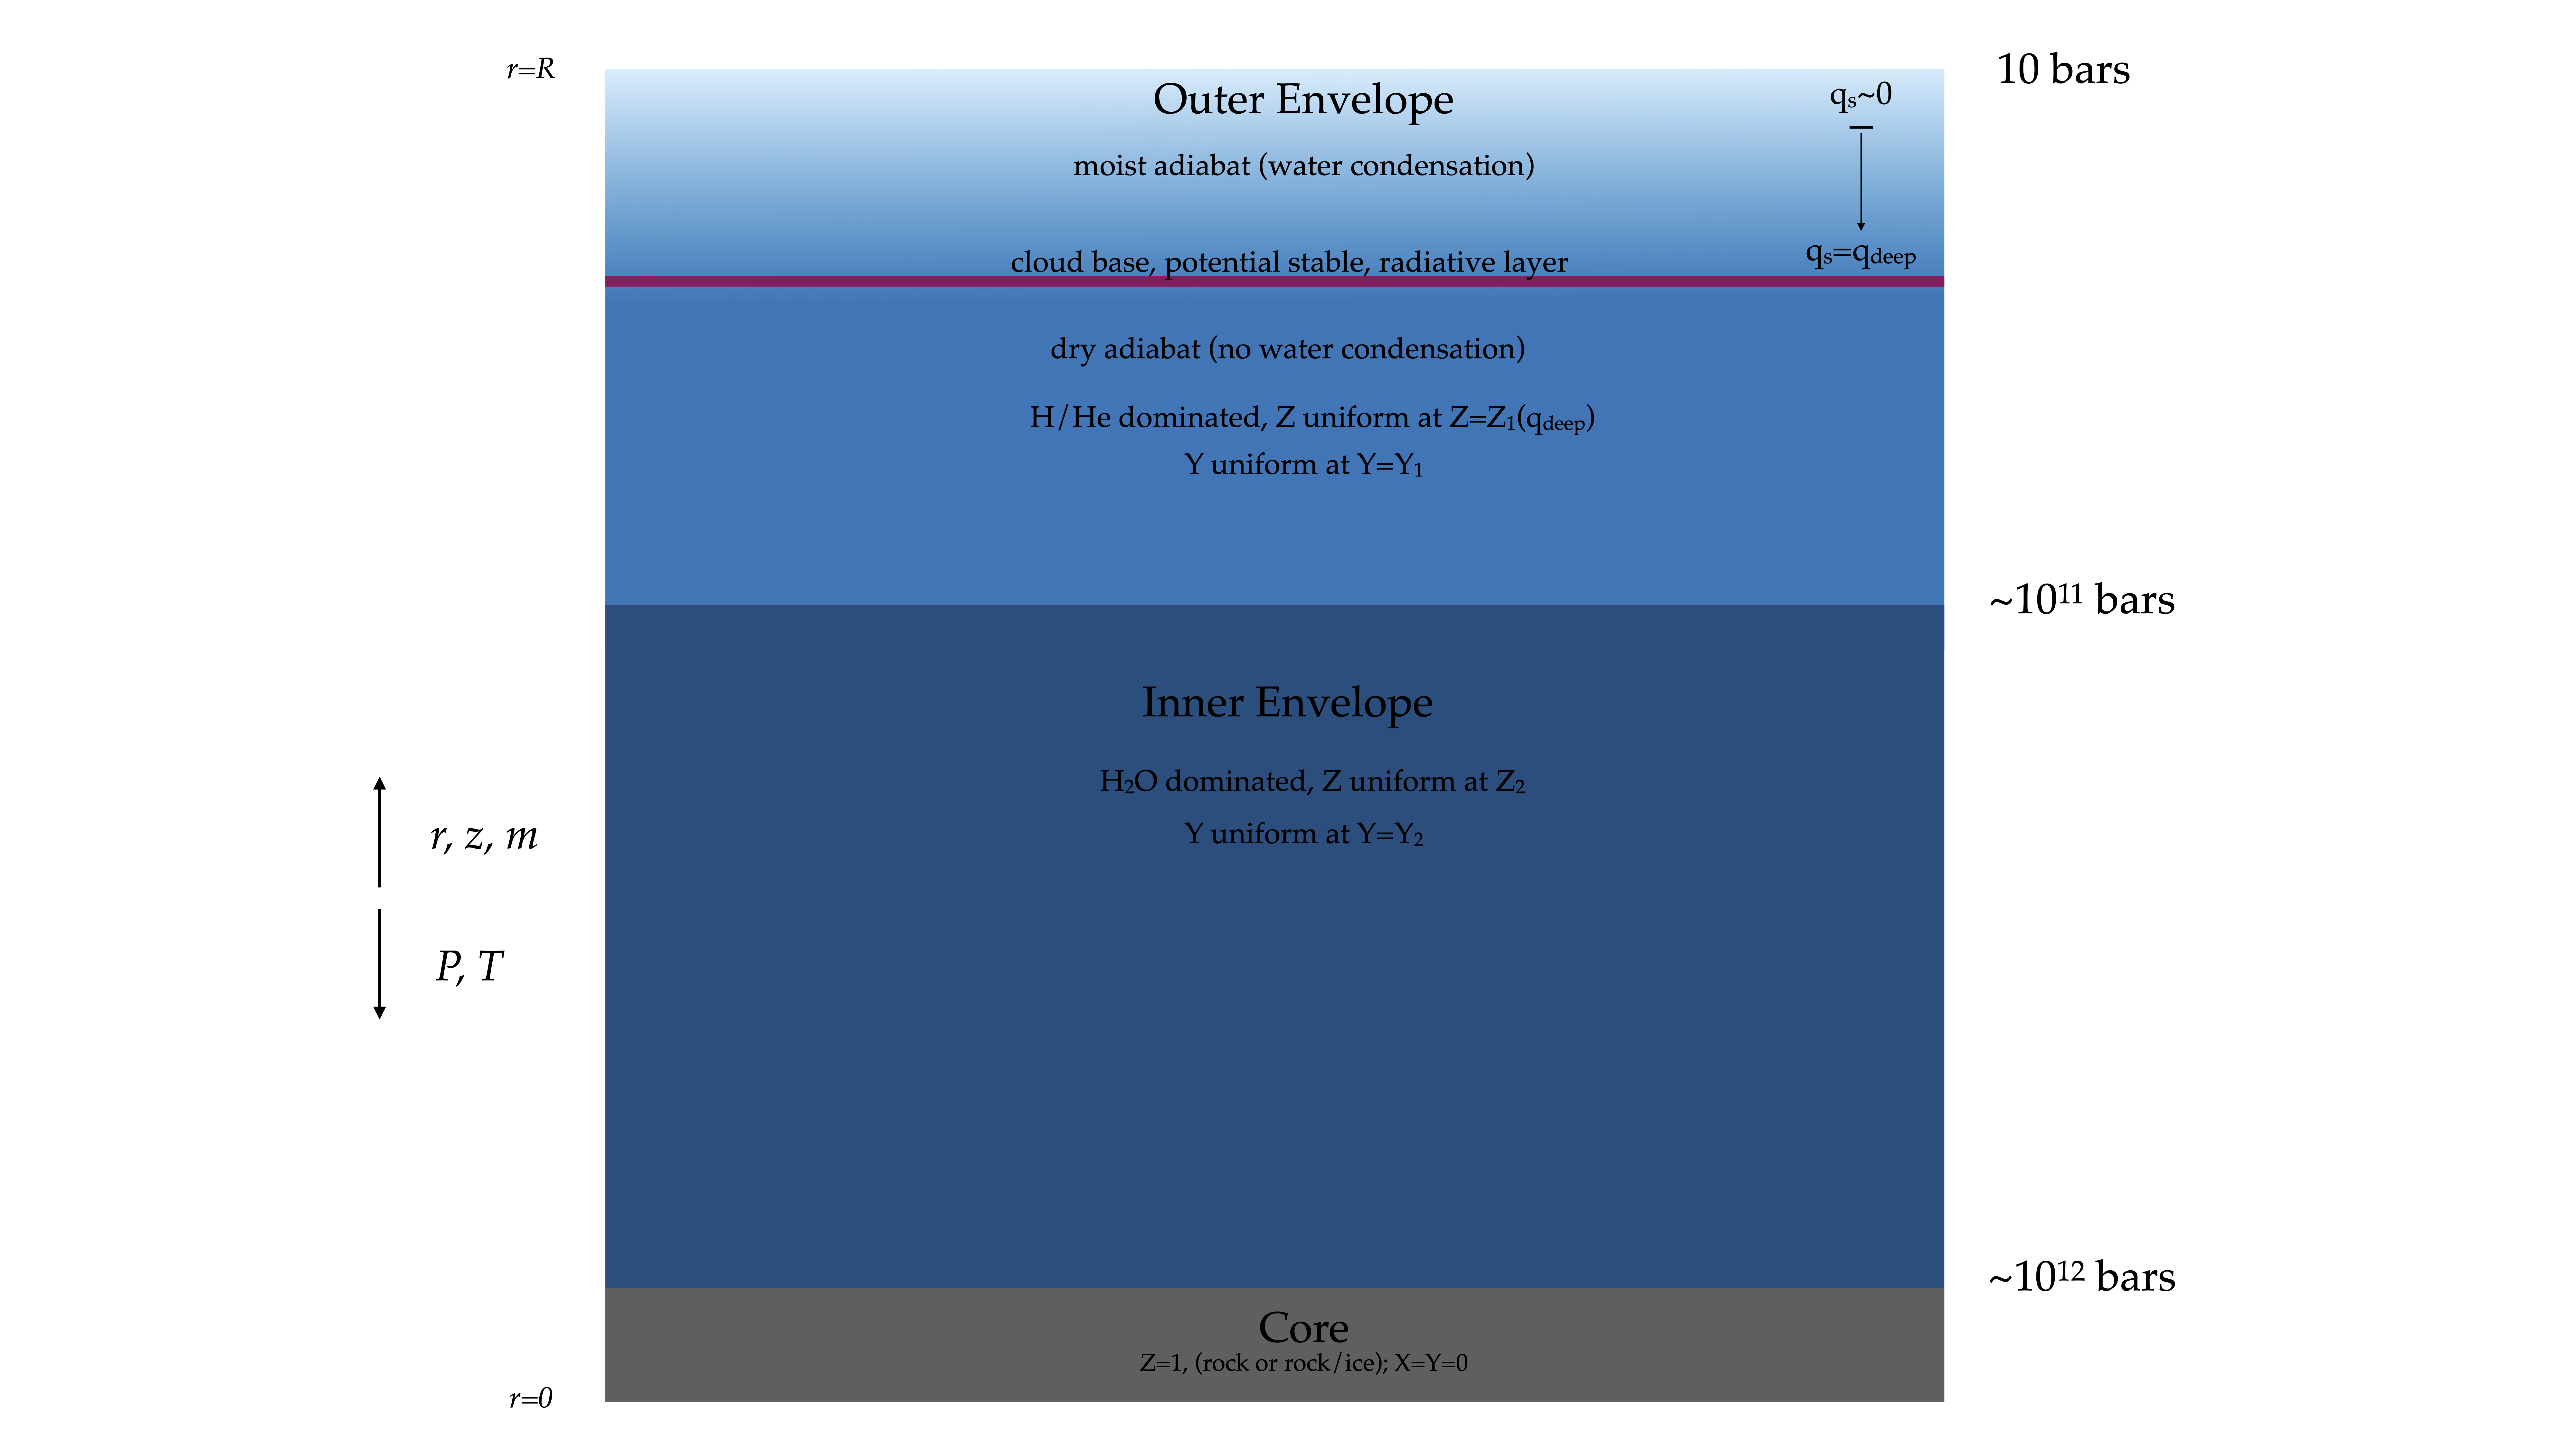
\includegraphics[width=8.0in]{figures/moist_adiabat_structure.png}
 }
\caption[Interior Structure for Moist Adiabat]
{The structure for moist adiabatic interior, allowing for condensation-inhibited convection.}
\label{fig:moist_interior}
\end{figure}


If condensation zone forms, it may be stable against convection. Convection is inhibited due to the formation of a stable condensation zone when $\alpha < 1$, where is $\alpha$ \citep{friedson_2017} is given by:

\begin{equation}
  \alpha = 1 + \xi (q_{s} L / R_{W} T_{0}) 
\end{equation}

If condensation is found to be inhibited,  

At pressure where $\alpha < 1$, the cloud base of the water condensation zone forms. This thin, stable radiative layer has a temperature profile that is governed by:

\begin{equation}
	T(P) = T_{\rm top} + \int_{P_{\rm top}}^P\left(\frac{dT}{dP}\right)_{\rm rad}\,d P
\end{equation}

\begin{equation}
  \left(\frac{dT}{dP}\right)_{\rm rad}=\frac{T}{P}\nabla_{\rm rad} = \frac{T}{P}\times\frac{3}{16}\frac{\kappa_R P}{g}\frac{T_{\rm int}^4}{T^4}
\end{equation}

\begin{equation}
	T_{\rm base}\equiv T(P+\Delta P) = T_{\rm top} + \left(\frac{dT}{dP}\right)_{\rm rad}\Delta P.
\end{equation}

\begin{equation}
	x_{\rm vap}(P, T) = x_{\rm vap}^{\rm sat}(P, T) = \frac{e_s(T)}{P}, \qquad P<P_{\rm base}.
\end{equation}

\begin{equation}
x_{\rm vap}^{\rm sat}(P_{\rm base}, T_{\rm base}) = \frac{e_s(T_{\rm base})}{P_{\rm base}}=x_{\rm vap}^{\rm deep}
\Longrightarrow \Delta P \equiv P_{\rm base}-P_{\rm top} = \frac{e_s(T_{\rm base})}{x_{\rm vap}^{\rm deep}} - P_{\rm top}
\end{equation}

\begin{equation}
	T_{\rm base} = T_{\rm top} + \left(\frac{dT}{dP}\right)_{\rm rad}\left(\frac{e_s(T_{\rm base})}{x_{\rm vap}^{\rm deep}} - P_{\rm top}\right)
\end{equation}

Below the base of the radiative layer, the temperature-pressure profile again follows a dry adiabat, given by Equation (2.1).



% \begin{figure}%
%     \centering
%     \subfloat[\centering The interiror structure for dry adiabat. This can also represent the situation in which the water condensation zone has eroded and the interior becomes fully convective. ]{{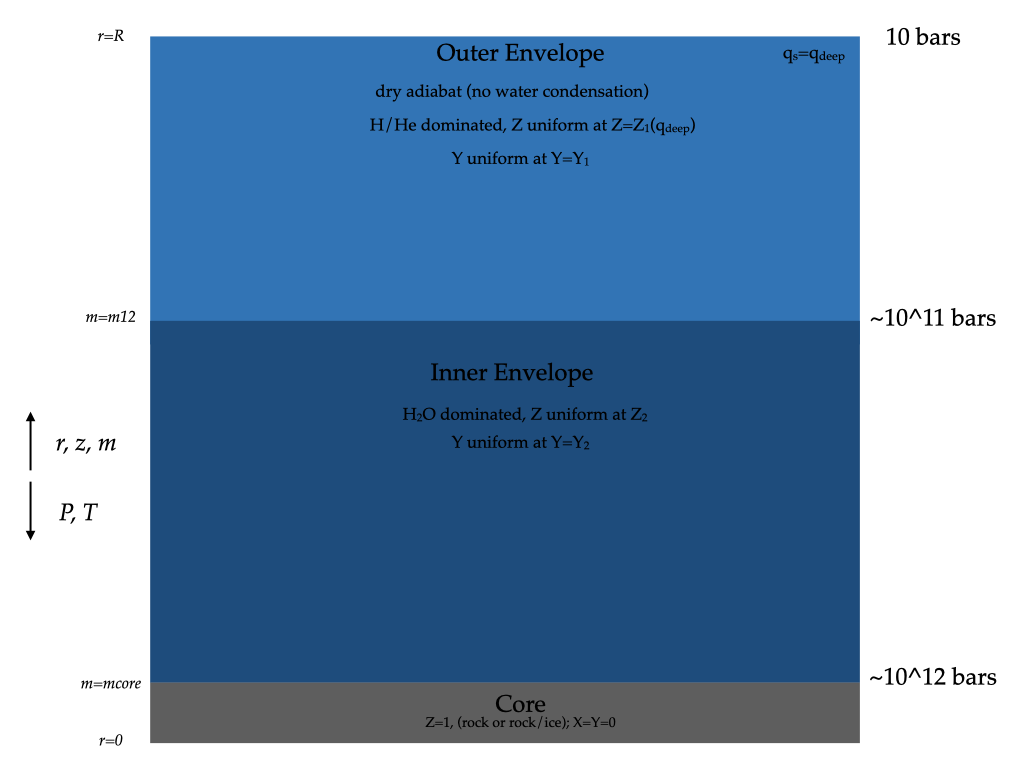
\includegraphics[width=12cm]{figures/structure_schematic_images/structure_schematic_images.001} }}%
%     \qquad
%     \subfloat[\centering The interior structure when a condensation zone has formed, creating a potentially stable, radiative layer. This represents the cloud base. It's depth decreases with a decrease in $T_{10}$. ]{{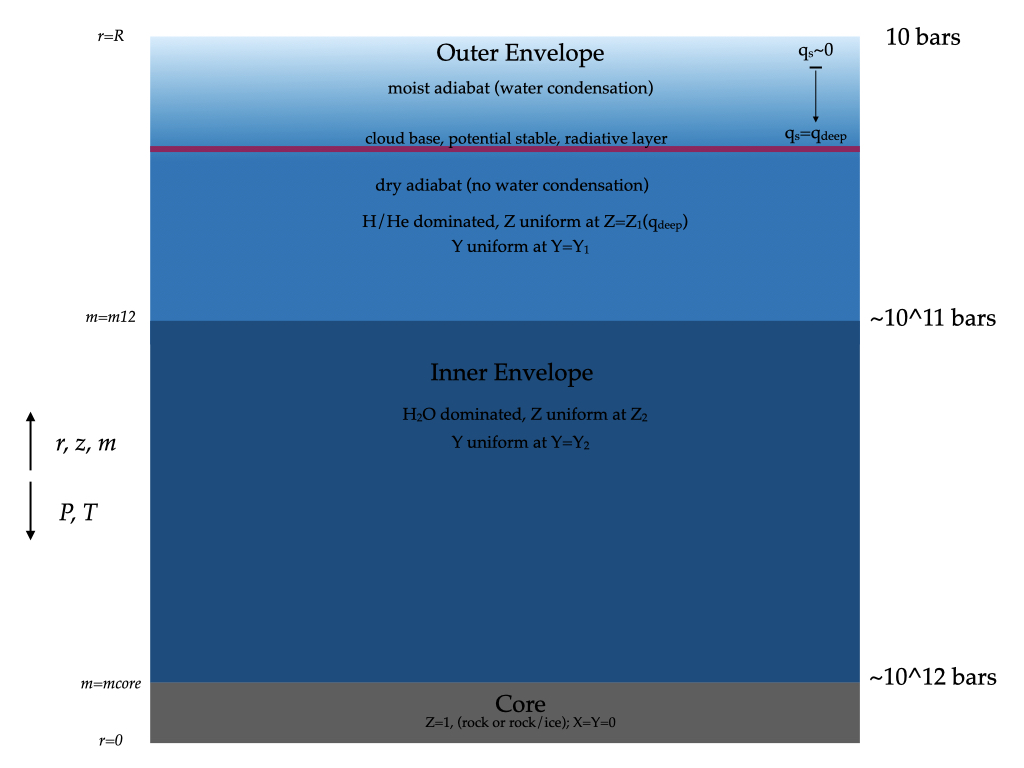
\includegraphics[width=12cm]{figures/structure_schematic_images/structure_schematic_images.002} }}%
%     \caption{Interior structure model for Uranus}%
%     \label{fig:example}%
% \end{figure}

% \begin{figure}[ht!]
%  \centerline{
%   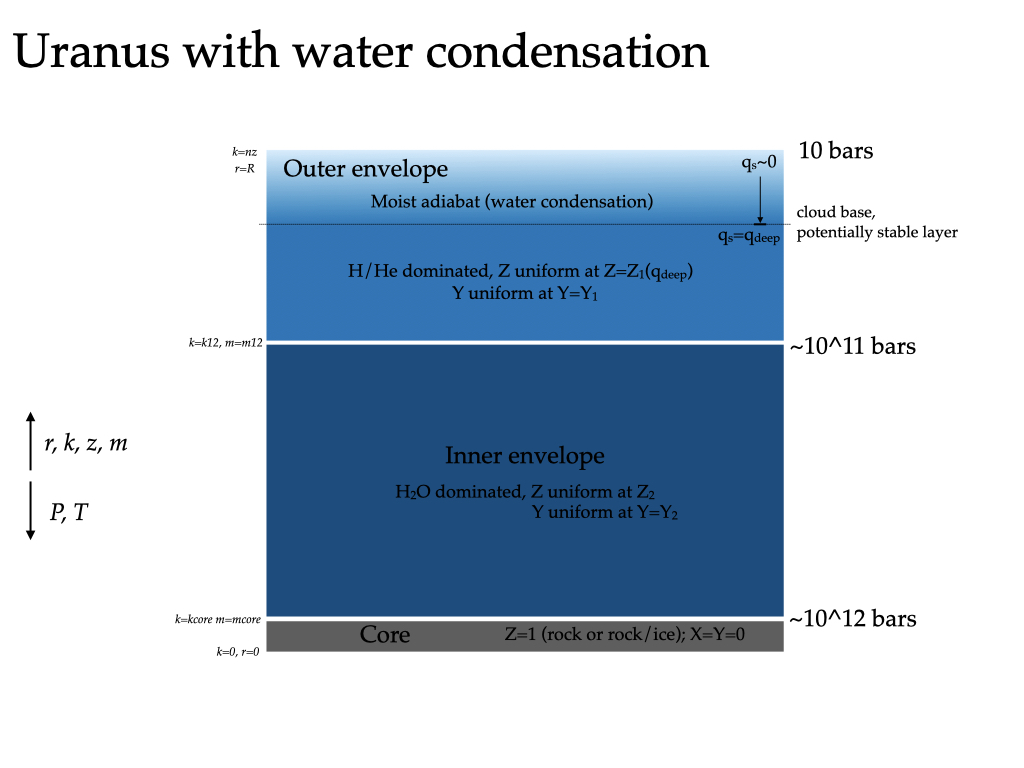
\includegraphics[width=7.0in]{figures/uranus_with_wcz_structure.001.jpeg}
%  }
% \caption[Interior Structure]
% {Model of interior structure of Uranus without condensation on the left and with condensation on the right. The dry adiabat model on the left can also represent the situation in which the water condensation zone has eroded and the interior becomes fully convective. The figure on the right shows the interior structure when a condensation zone has formed, creating a potentially stable, radiative layer. This represents the cloud base. It's depth decreases with a decrease in $T_{10}$.}
% \label{fig:uranus}
% \end{figure}



\chapter{Results}

\section{Condensation-inhibited Convection}
Talk about Figure 3.1.
\begin{figure}[ht!]
 \centerline{
  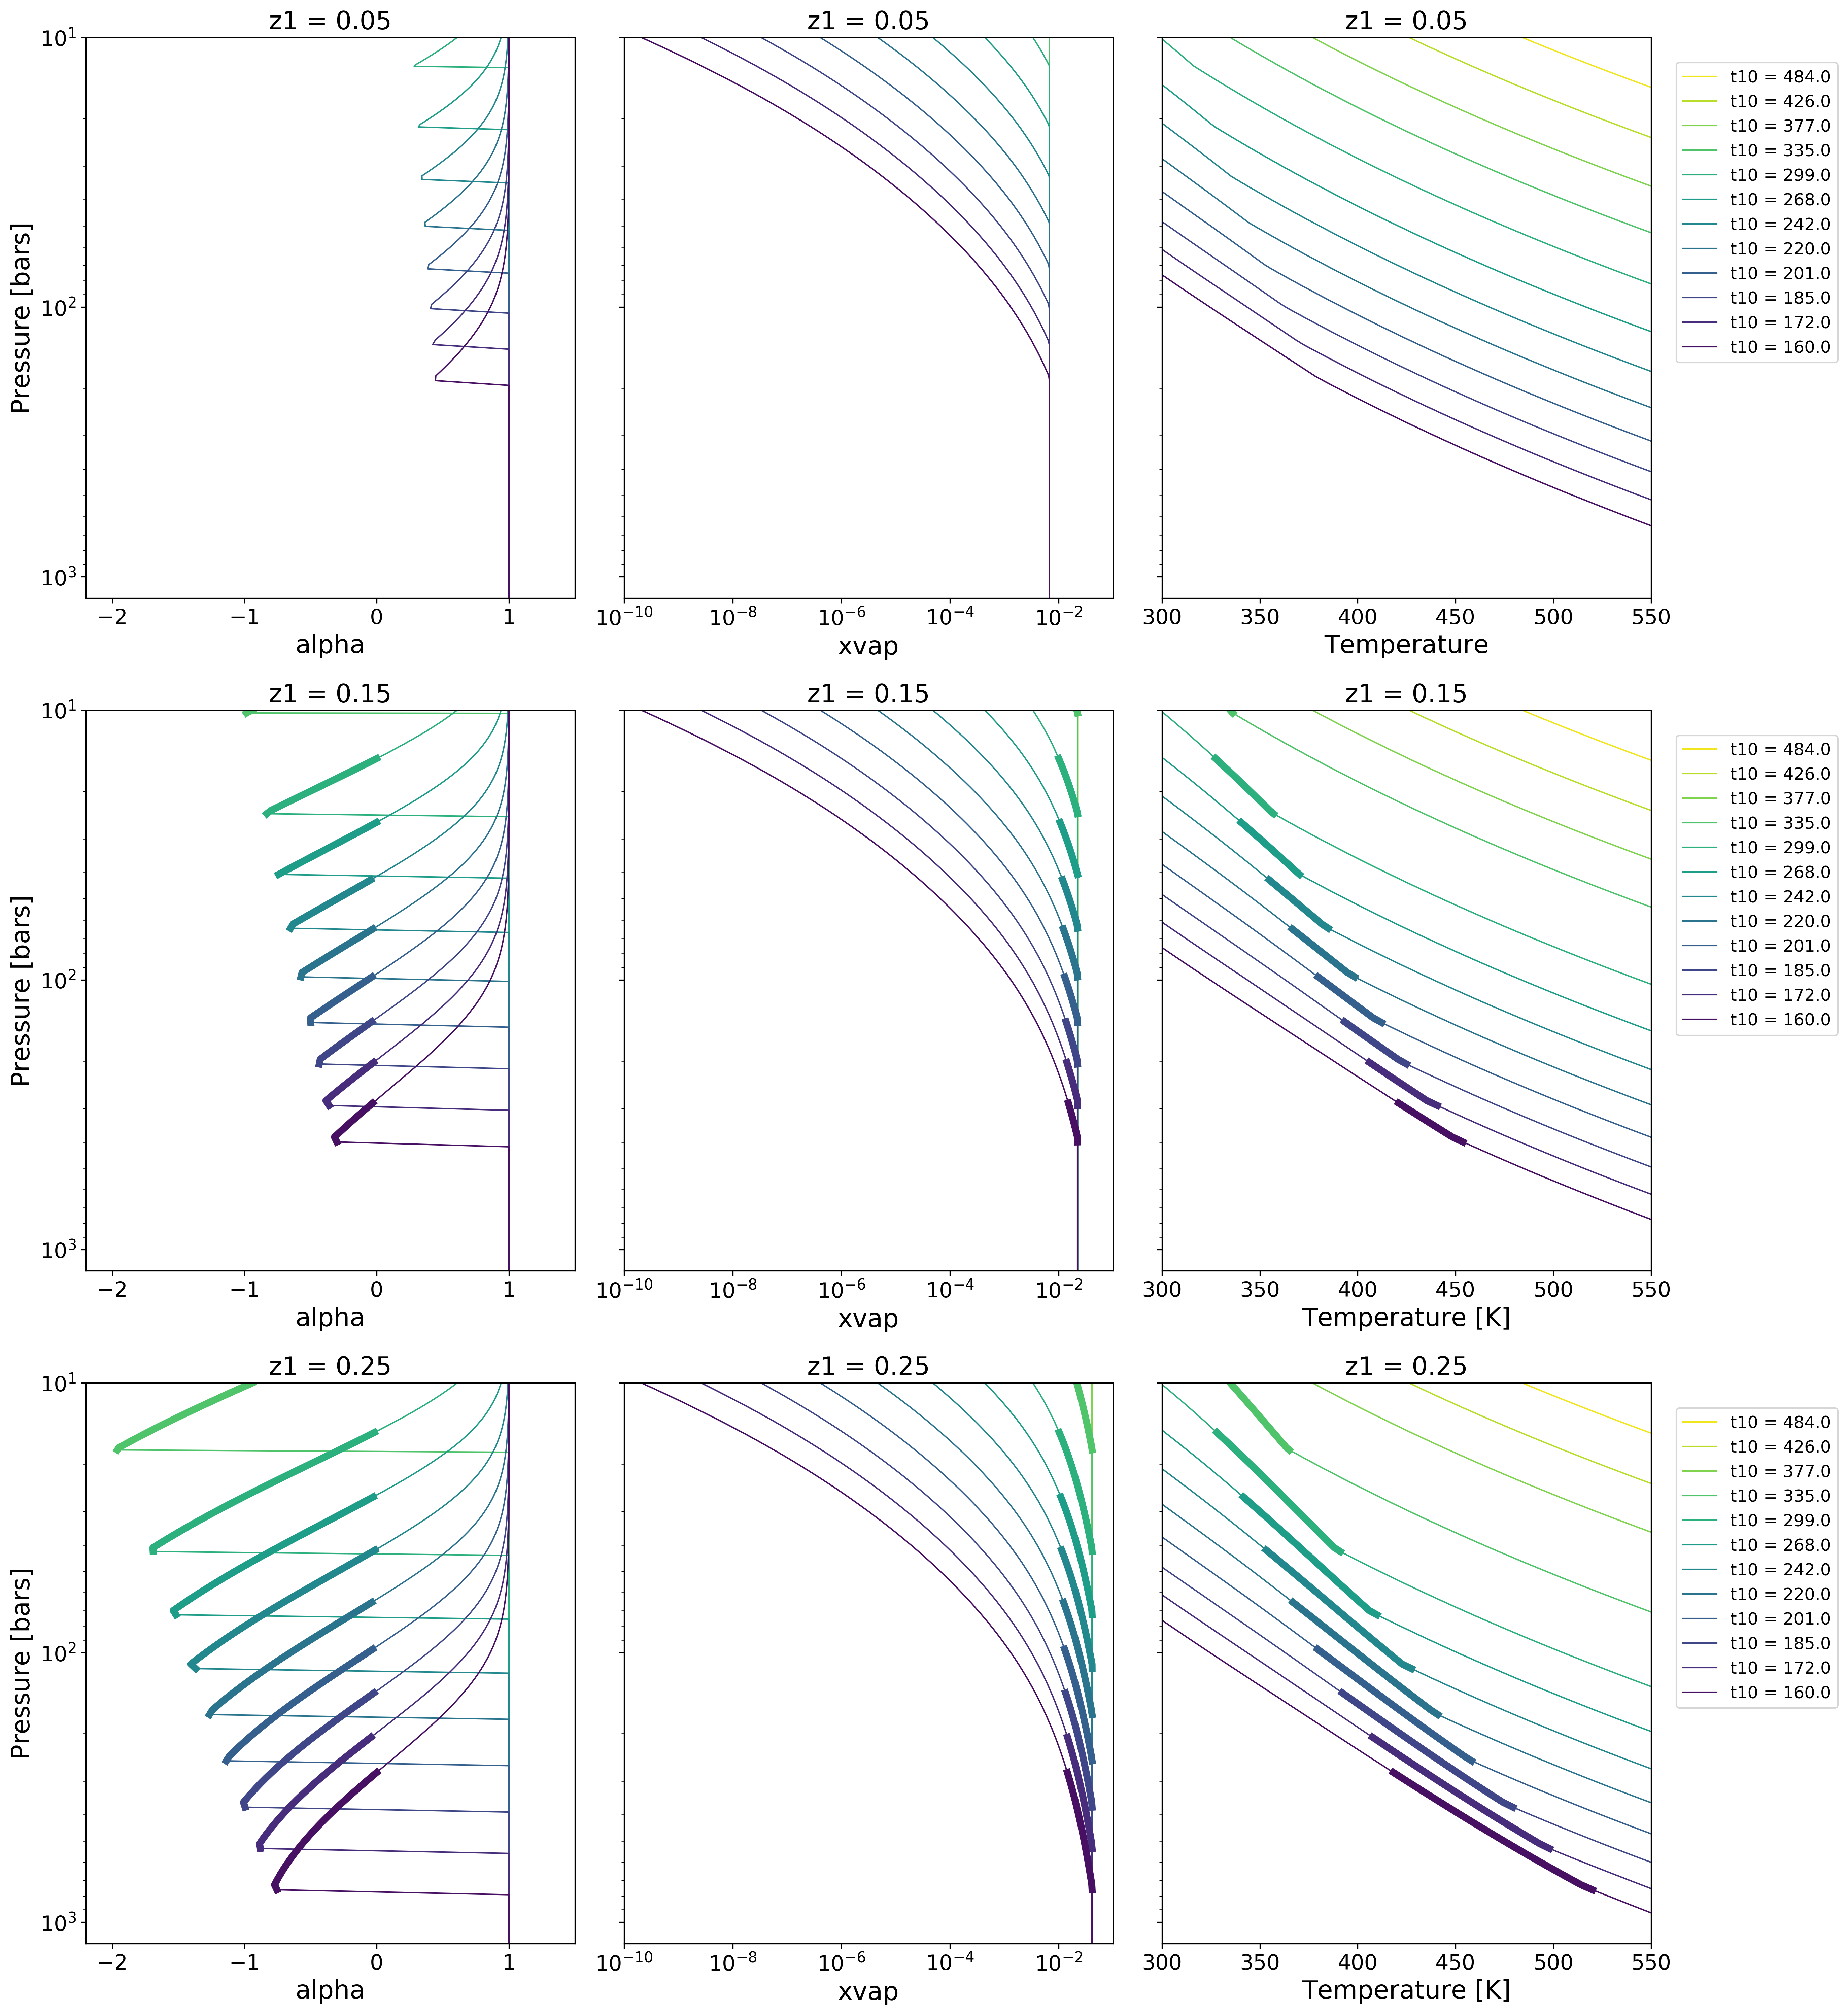
\includegraphics[width=7.0in]{figures/convection_inhibited_2.png}
 }
\caption[Inhibition of convection on Uranus]
{add description re: moist adiabat, when/where convection is inhibited and where the radiative zone base is in these plots. explain differences}
\label{fig:convection_inhibited}
\end{figure}



\section{Formation of Radiative Layer}
Talk about Figure 3.2.
\begin{figure}[ht!]
 \centerline{
  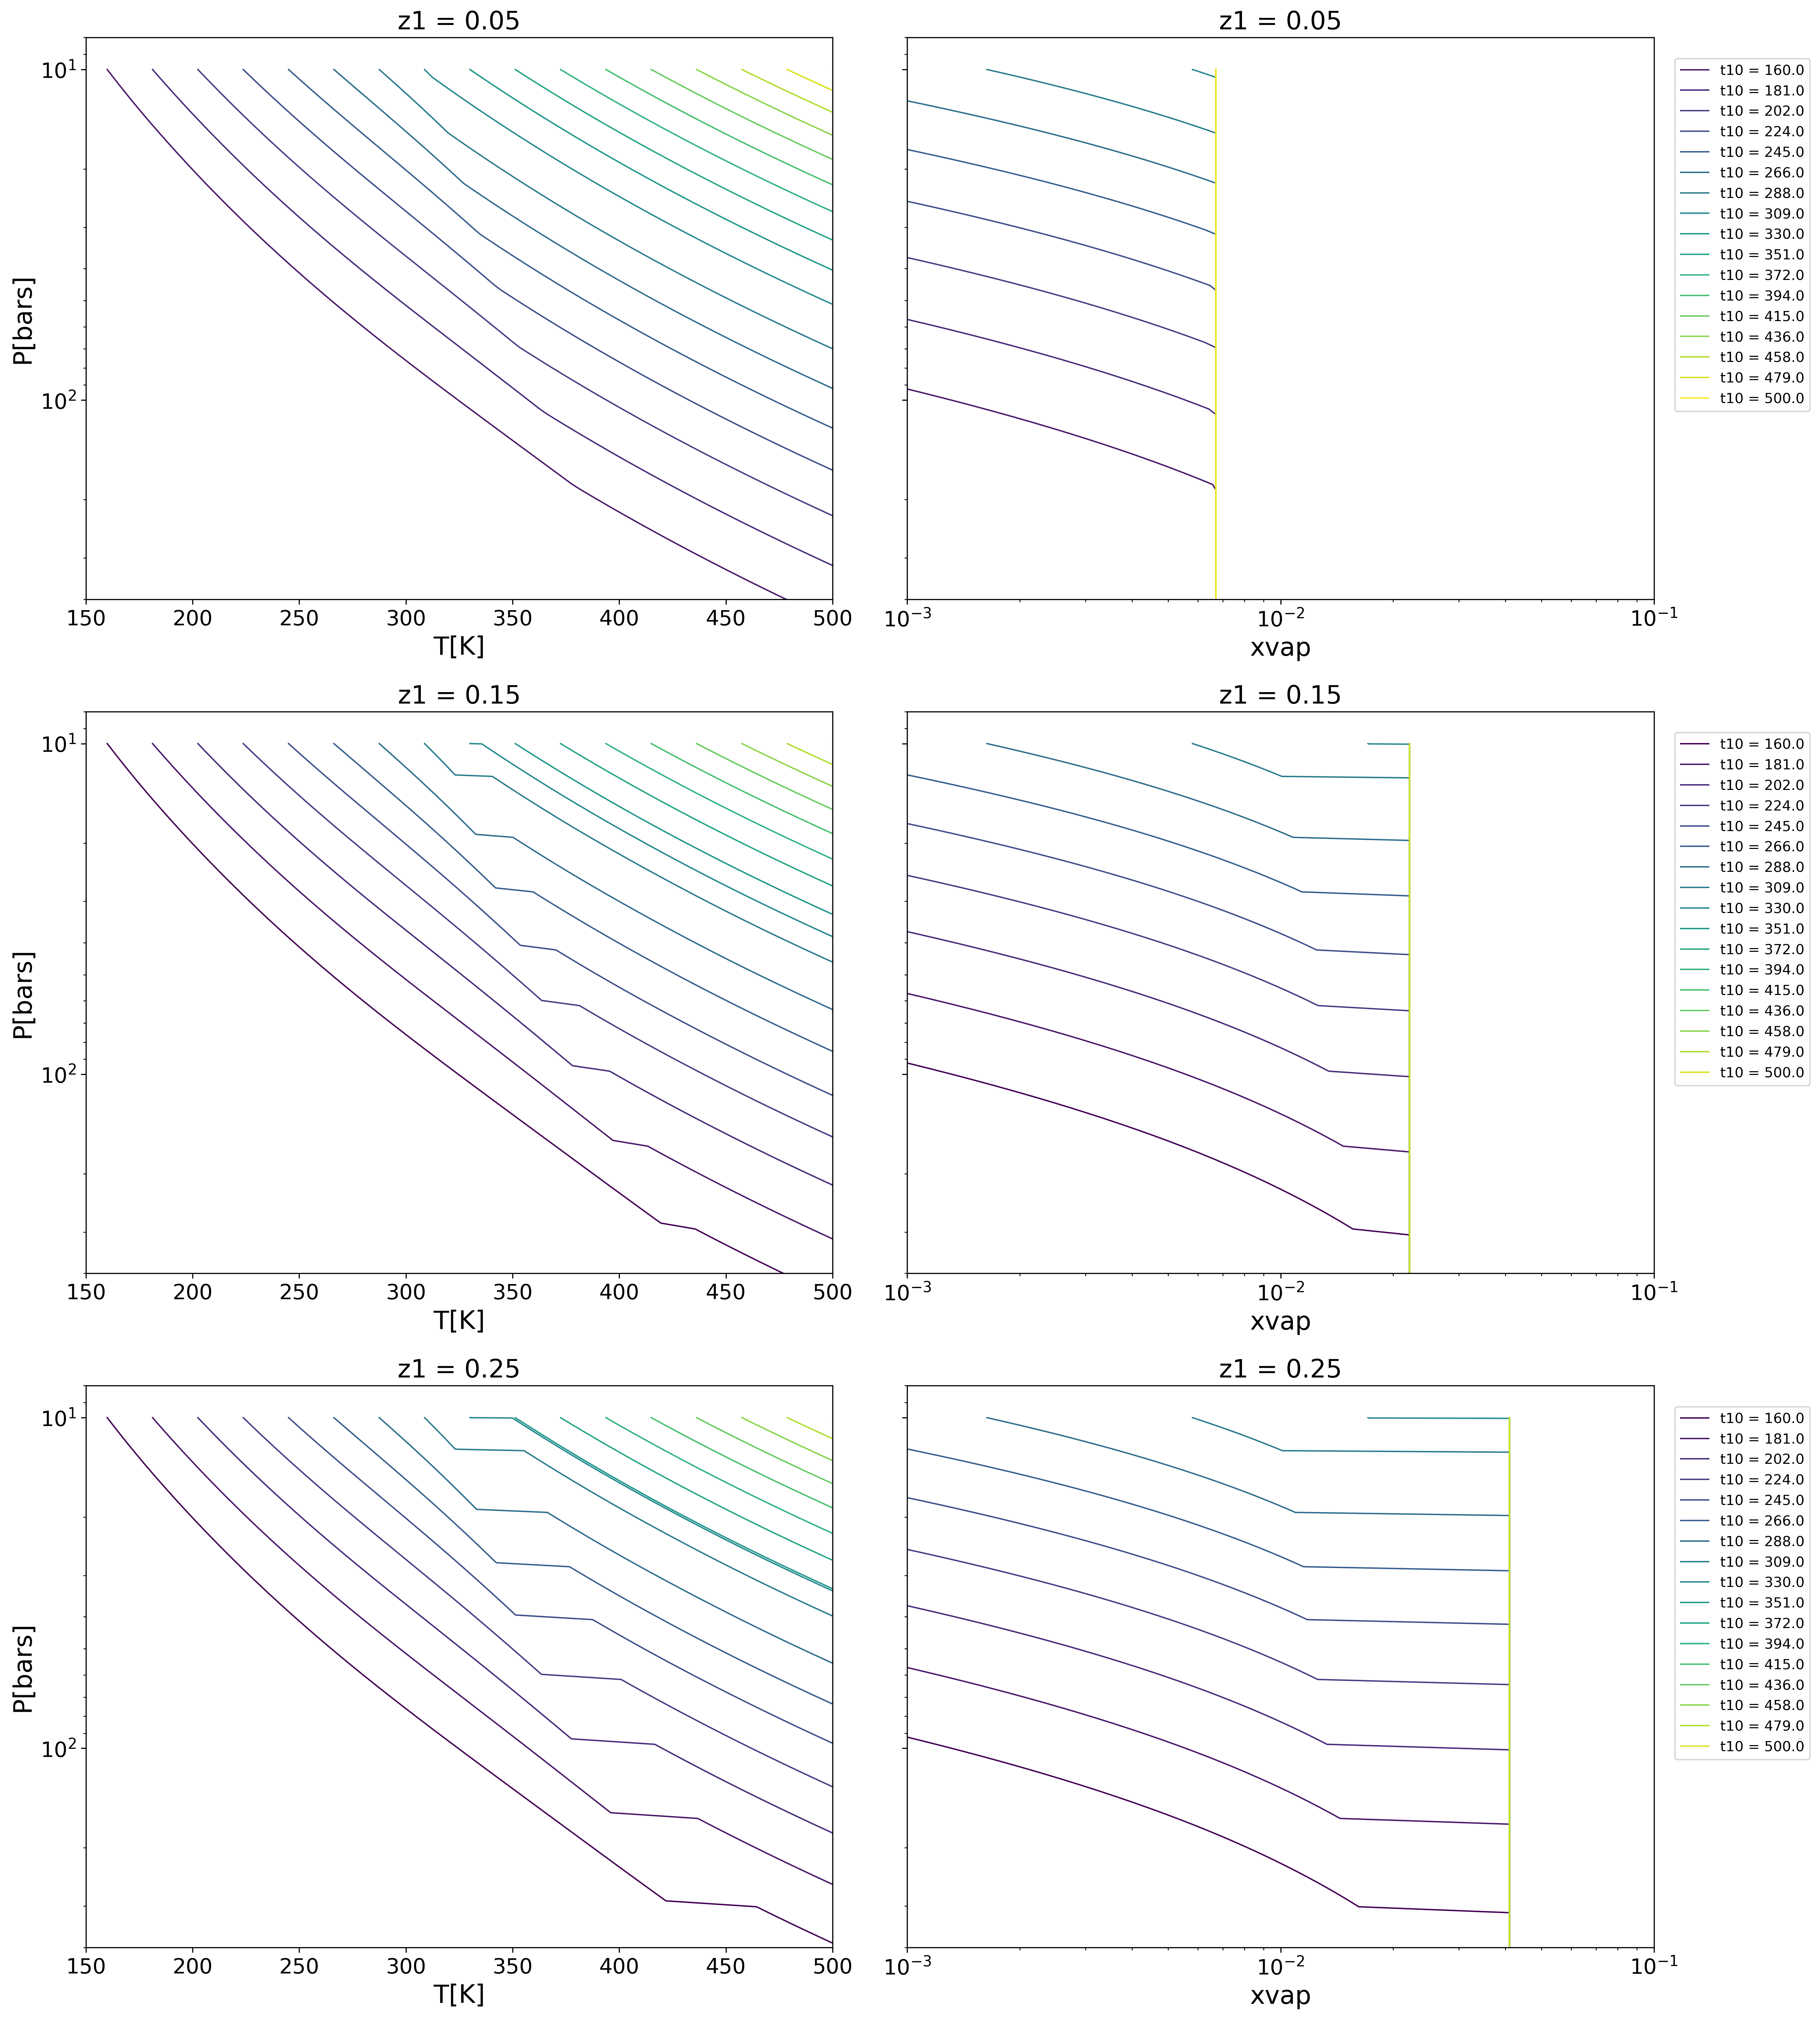
\includegraphics[width=7.0in]{figures/static_radiative_layer_plots_without_grid_points.png}
 }
\caption[Inhibition of convection on Neptune]
{add description these plots. explain differences}
\label{fig:radiative}
\end{figure}


\section{Thermal Evolution}
Talk about Figure 3.3.



\chapter{Discussion and Conclusions}





\appendix
\chapter{Some Ancillary Stuff}


\bibliography{wcz_bib}


\end{document}
